\subsection{MainControl}
MainControl er klassen, som er bindeleddet mellem klienter og database. Det er i MainControl, at alt serverens kontrol logik ligger placeret. MainControl tager imod kommandoer fra klienter og kan evt. svare/broadcaste kommandoer ud til alle forbundne klienter.\\

MainControl implementerer interfacet IMessageHandler, således at den kan håndtere beskeder modtaget fra andre tråde.\\

MainControl benytter tre interfaces: ISessionControl til håndtering af klienters sessioner, ILog til at skrive til log samt ICommandHandler til at håndtere kommandoer, som er modtaget fra klienter.

\begin{figure}[H]
    \centering
    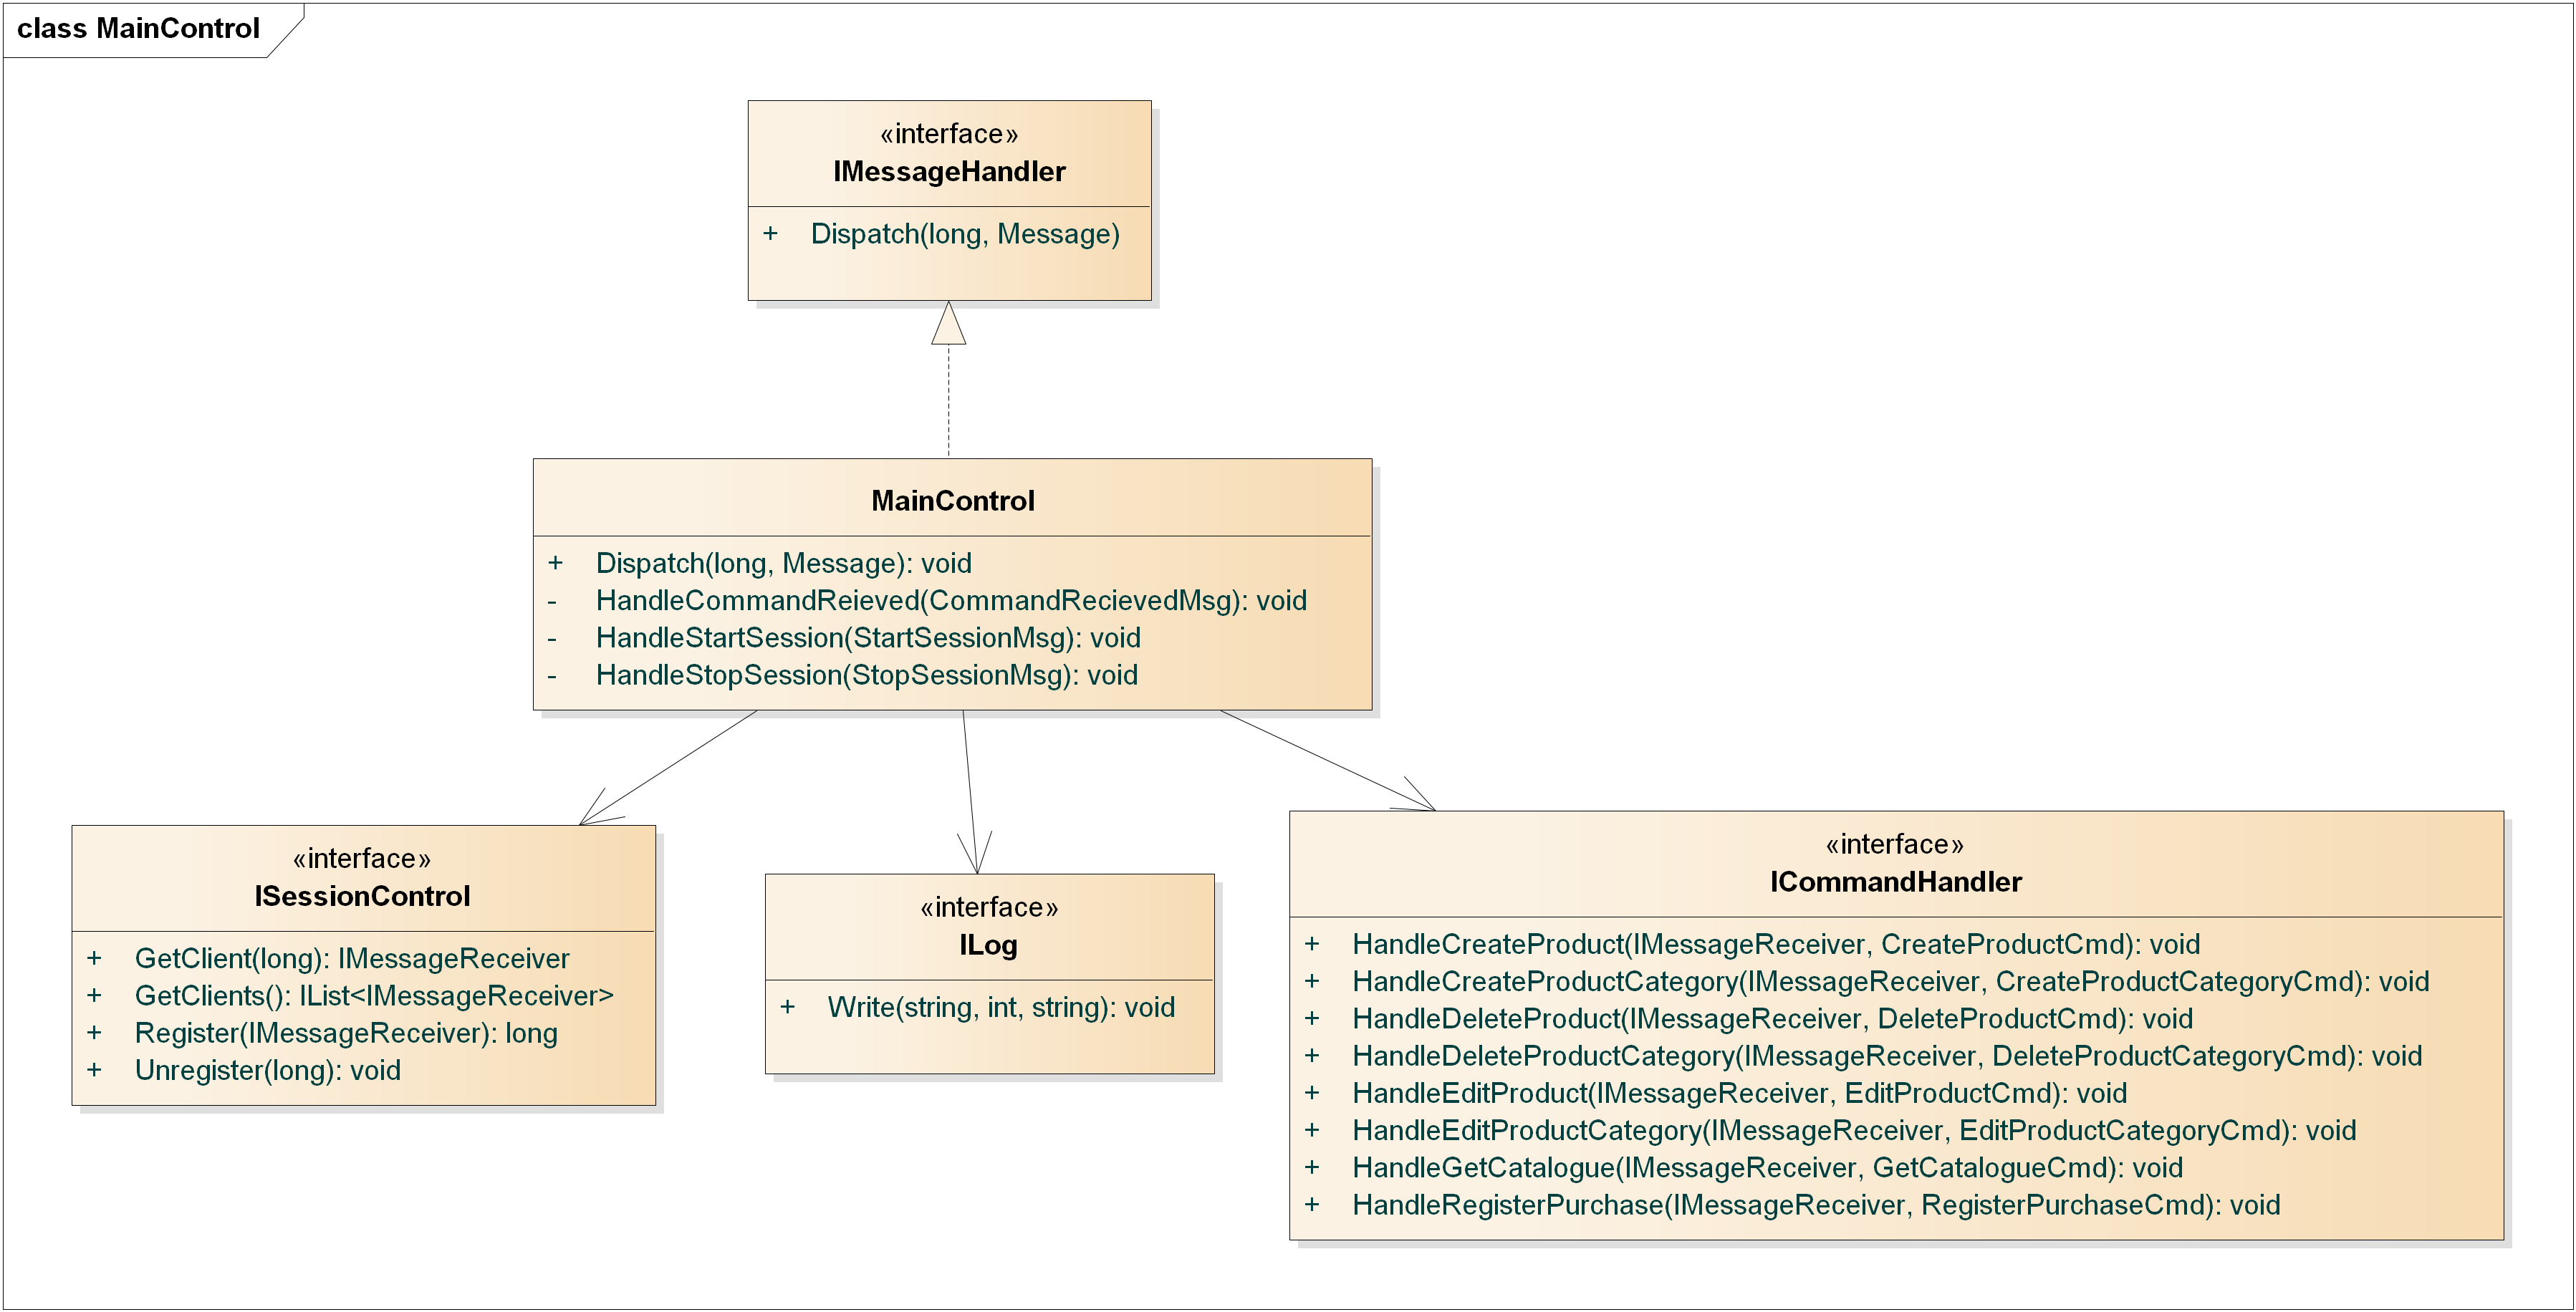
\includegraphics[width=1\textwidth]{Systemdesign/CentralServer/Images/MainControl.png}
    \caption{UML-diagram for MainControl}
    \label{fig:CSMainControl}
\end{figure}


\textbf{Events}\\
MainControl kan modtage følgende events:\\

\textbf{E\_START\_SESSION}:
Modtages når en klient er forbundet, og ønsker at registrere sig hos MainControl. Når MainControl modtager denne besked, så registreres en ny session. Indeholder attributten Client, som MainControl kan sende beskeder tilbage til. MainControl svarer tilbage til klienten med en WelcomeMsg, som indeholder klientens unikke sessions id.\\

\textbf{E\_STOP\_SESSION}:
Modtages når en klient har lukket forbindelsen til serveren, så MainControl ved, at klienten ikke længere er forbundet.\\

\textbf{E\_COMMAND\_RECEIVED}:
Modtages når en klient har sendt en kommando. MainControl afgører hvilken kommando der modtages og kalder den tilsvarende funktion på ICommandHandler.\\


\textbf{Sessions}\\
En session repræsenterer en klient, som er forbundet til serveren. Det benyttes af MainControl til at holde styr på, hvilke klienter, der er forbundet til serveren samt at kunne adskille dem. MainControl benytter ISessionControl til at håndtere klienters sessions.\\

En session består af et unikt sessions id samt en reference til klienten, som har det sessions id.\\

Når MainControl modtager en besked fra en klient kan MainControl identificere klienten vha. dens sessions id.\\


\textbf{Håndtering af kommandoer}\\
MainControl benytter sig at en ICommandHandler til at håndtere kommandoer modtaget fra klienter. Interfacet stiller en funktion (handlers) til rådighed for hver kommando serveren kan modtage fra klienter.\\

Hver funktion i interfacet tager imod to parametre:

\begin{itemize}
  \item En IMessageReceiver, som repræsenterer klienten, der sendte kommandoen. Handleren kan benytte dette objekt til at sende data tilbage til klienten. 
  \item Et kommando-objekt svarende til den kommando, klienten sendte.
\end{itemize}



\begin{figure}[H]
    \centering
    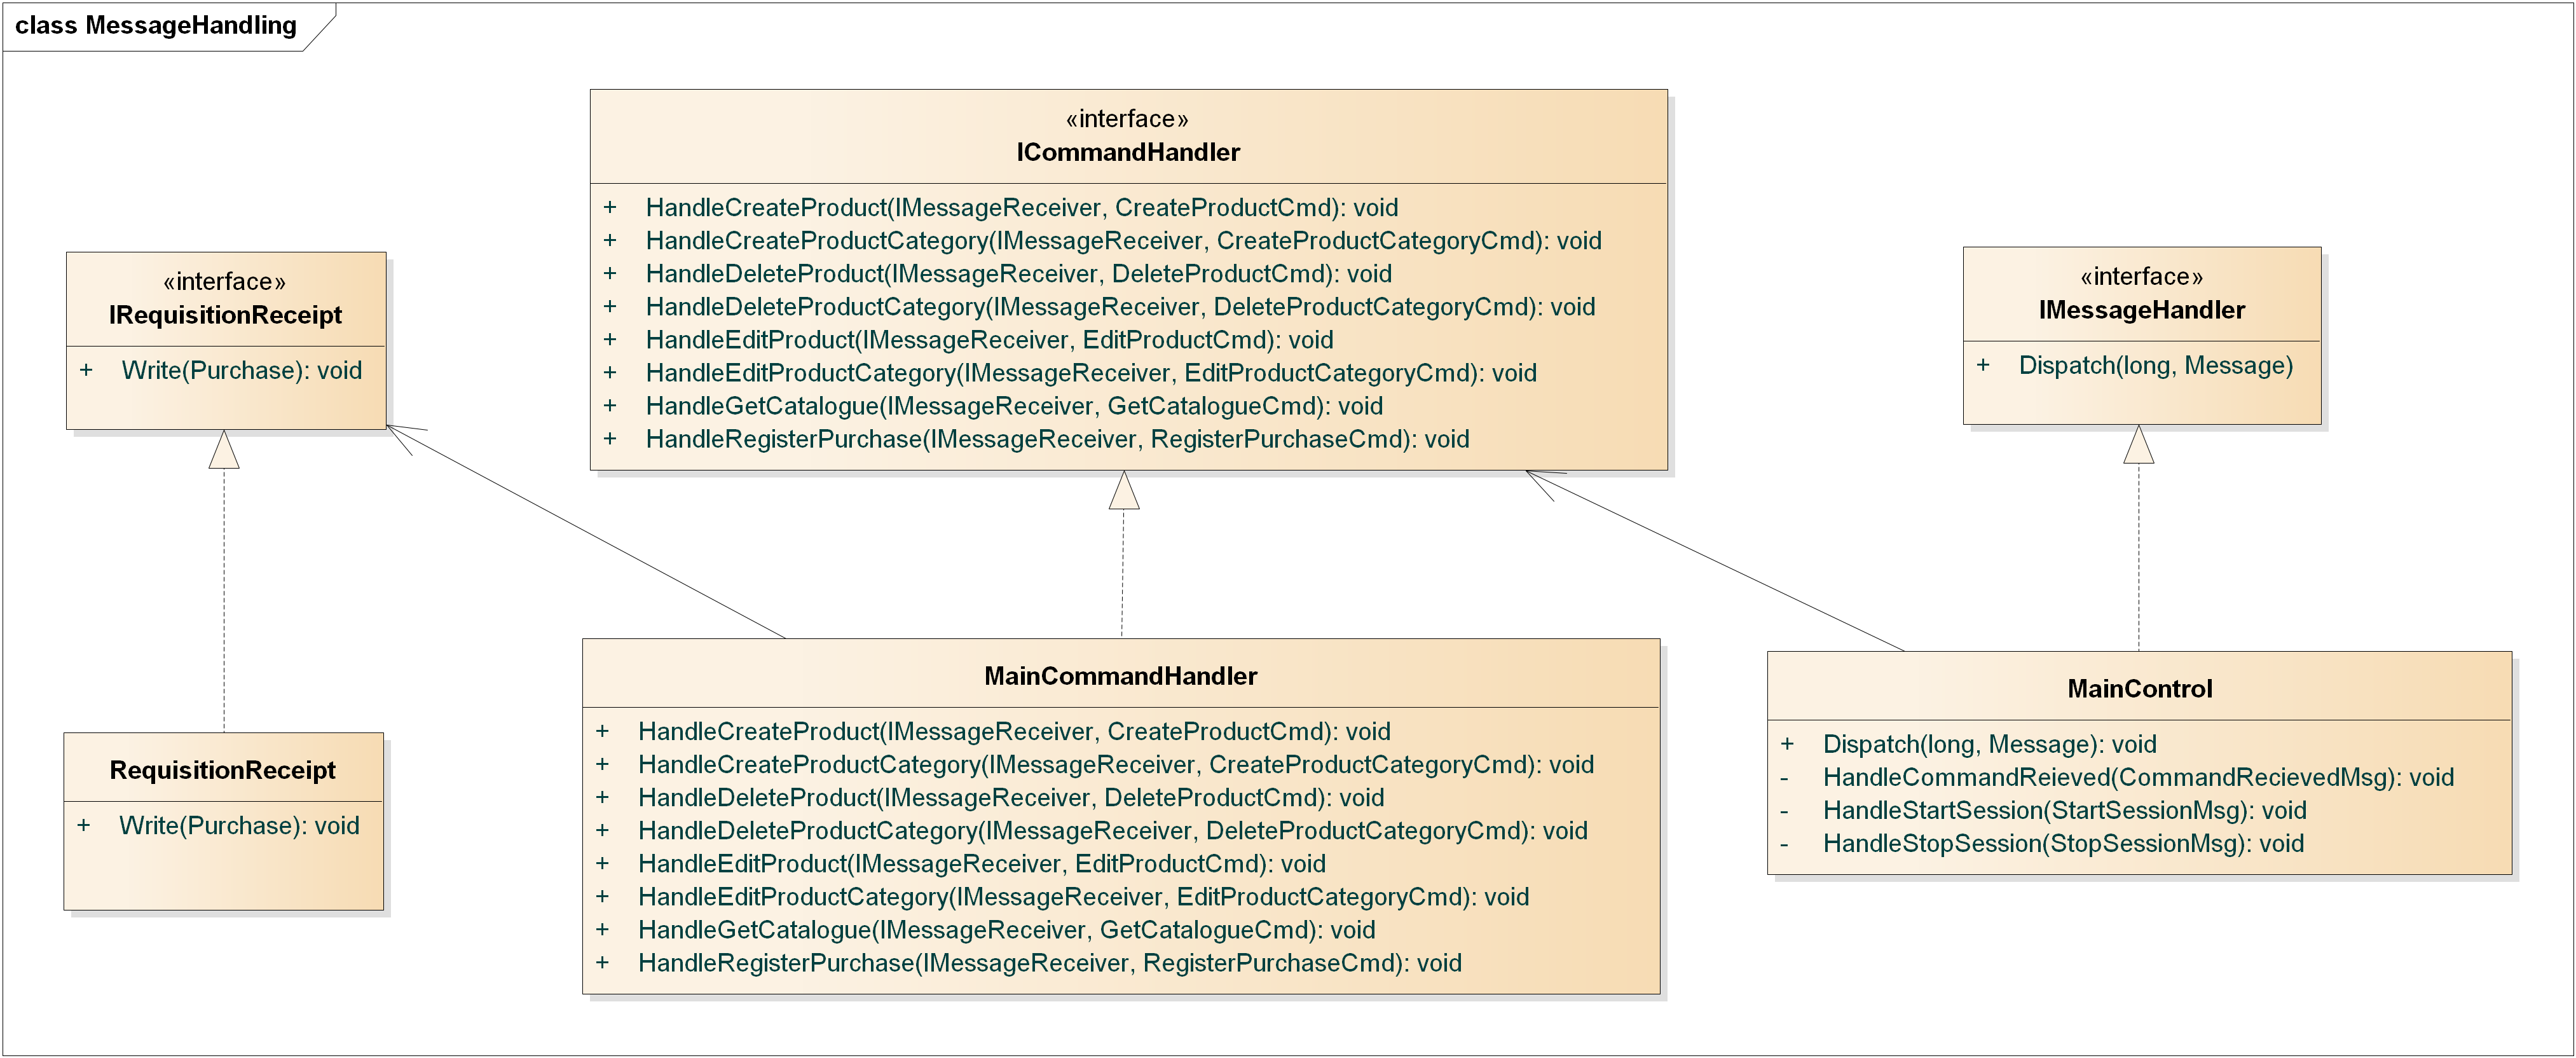
\includegraphics[width=1\textwidth]{Systemdesign/CentralServer/Images/BeskedHaandtering.png}
    \caption{UML-diagram for beskedhåndtering i MainControl}
    \label{fig:CSBeskedHaandtering}
\end{figure}

\begin{figure}[H]
    \centering
    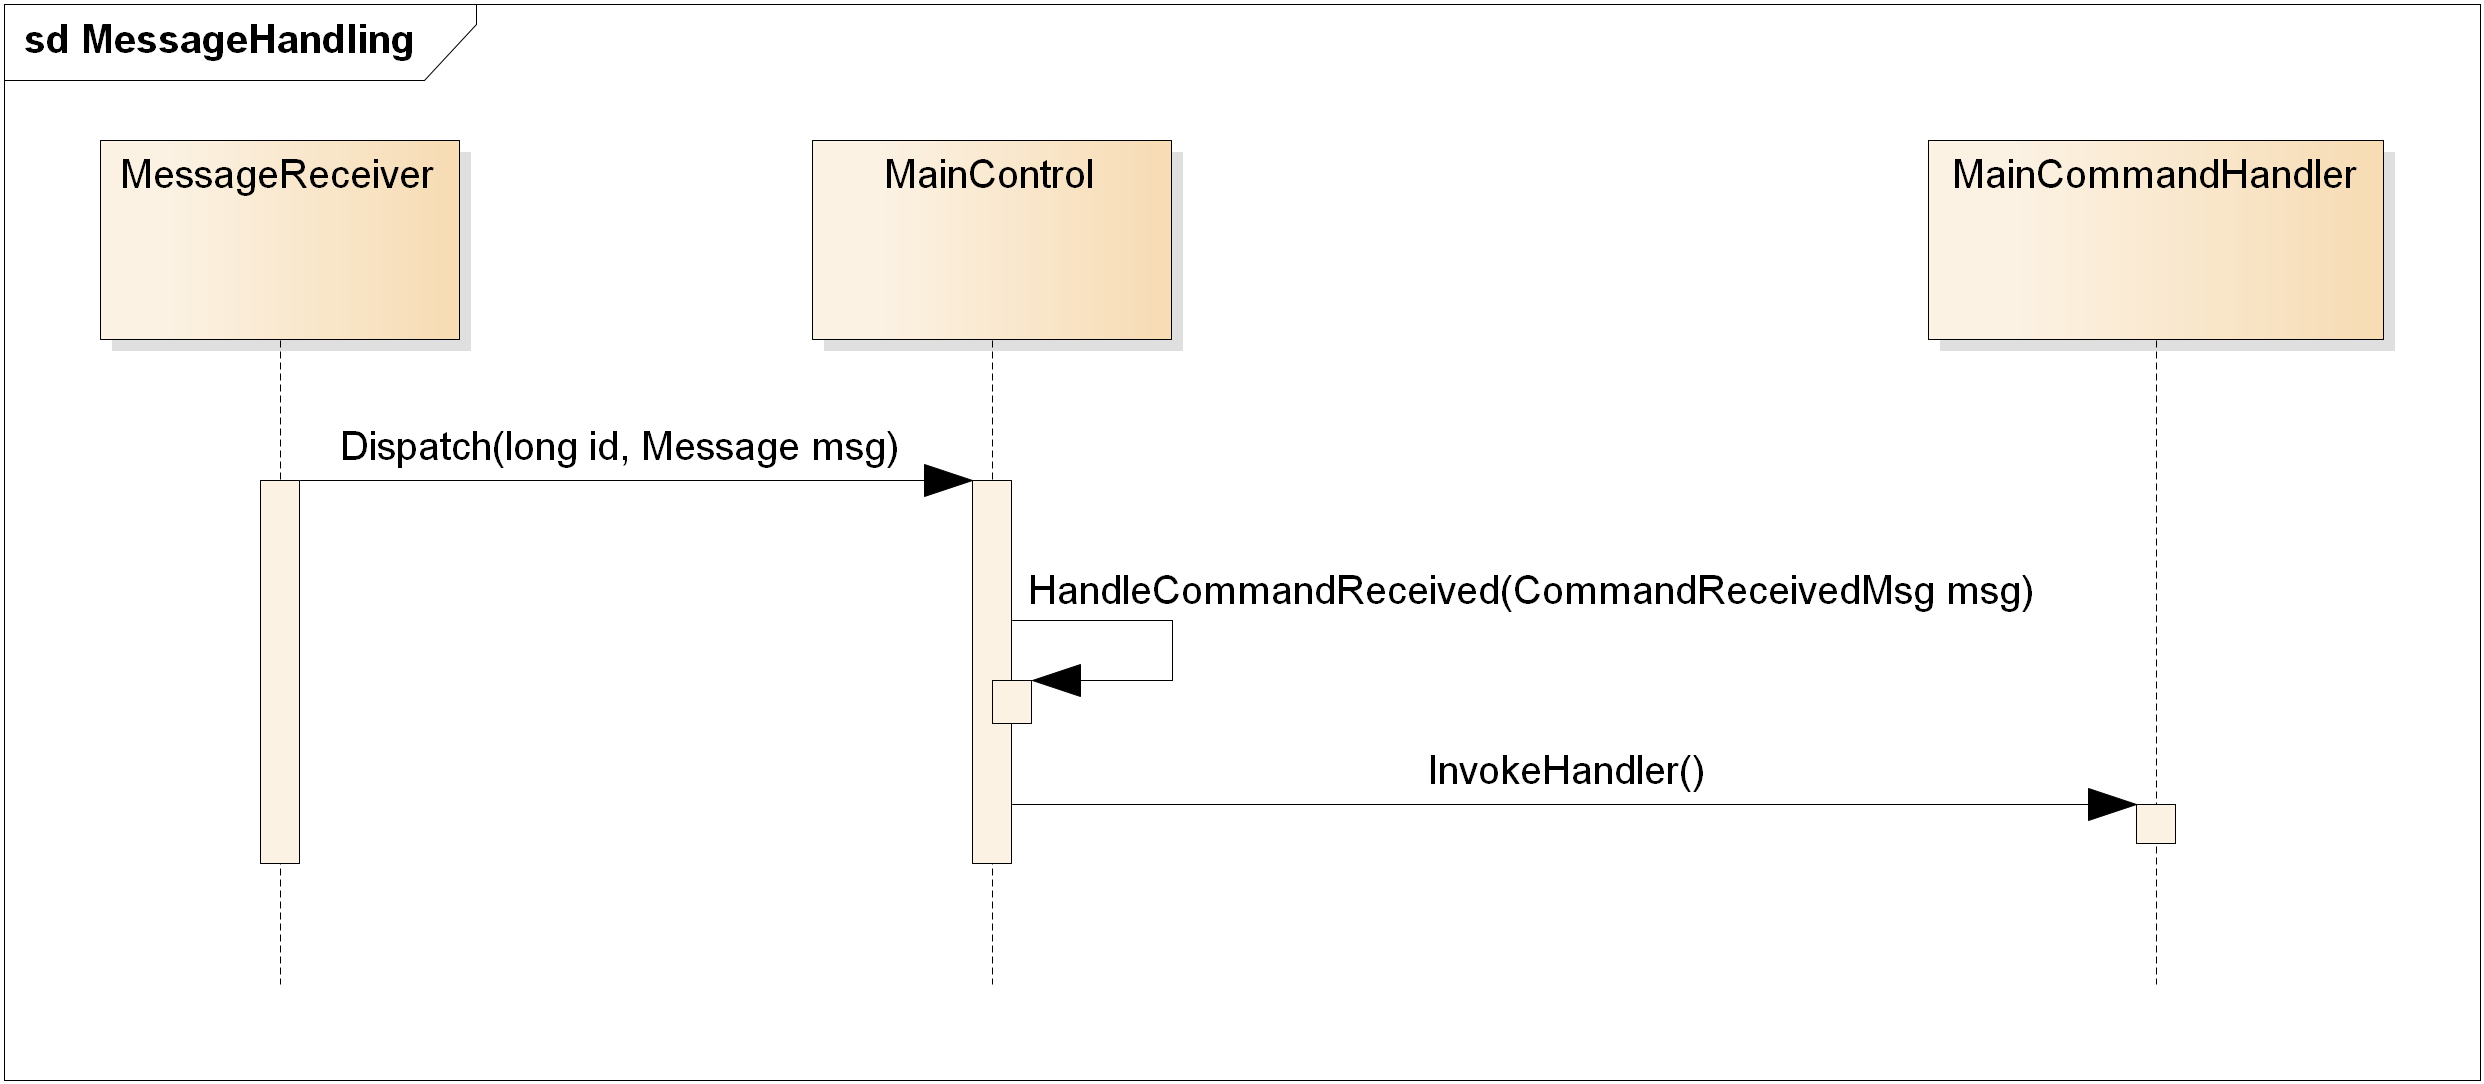
\includegraphics[width=1\textwidth]{Systemdesign/CentralServer/Images/BeskedHaandteringSekvens.png}
    \caption{Sekvensdiagrammet viser, hvordan MainControl håndterer kommandoer modtaget fra ClientControl}
    \label{fig:CSBeskedHaandteringSekvens}
\end{figure}


